\documentclass[tikz,border=8pt]{standalone}
\usepackage[utf8]{inputenc}
\usepackage{amsmath,amssymb}
\usepackage{microtype}
\usetikzlibrary{arrows.meta,calc,positioning}

\definecolor{maroon}{RGB}{122,36,53}
\definecolor{taupe}{RGB}{124,95,88}
\definecolor{gold}{RGB}{154,106,31}
\definecolor{muted}{RGB}{124,116,104}
\definecolor{rule}{RGB}{189,169,132}

\tikzset{>=Stealth}

\begin{document}
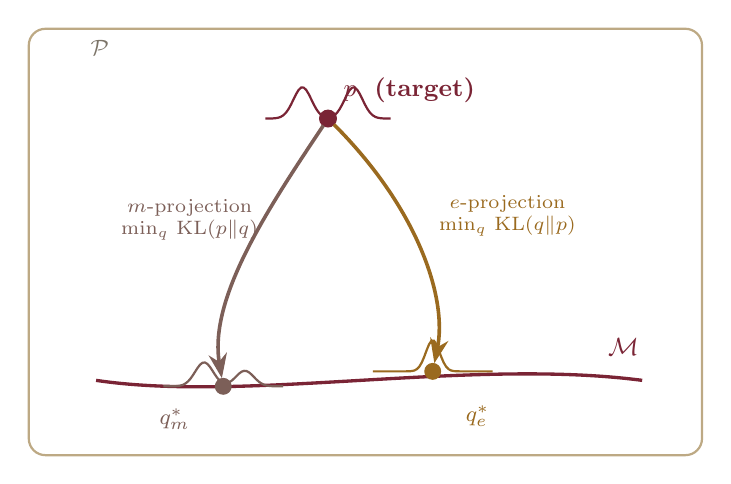
\begin{tikzpicture}[font=\small,scale=0.95]
  % Distribution space and model family
  \draw[rule,rounded corners=6pt,thick]
    (-0.4,-0.5) rectangle (8.6,5.2);
  \node[muted,font=\footnotesize\itshape] at (0.55,4.95)
    {$\mathcal P$};

  \draw[maroon,very thick]
    (0.5,0.5) .. controls (2.5,0.2) and (5.5,0.8) .. (7.8,0.5);
  \node[maroon,font=\small\itshape] at (7.55,0.95)
    {$\mathcal M$};

  % Target
  \coordinate (ptarget) at (3.6,4.0);
  \filldraw[maroon] (ptarget) circle (3.2pt);
  \node[maroon,above right=3pt,font=\small\bfseries]
    at (ptarget) {$p$\; (target)};

  \begin{scope}[shift={(ptarget)},scale=0.38]
    \draw[maroon,thick,domain=-2.2:2.2,samples=50]
      plot(\x,{1.1*(exp(-5*(\x+0.9)*(\x+0.9))
                    +exp(-5*(\x-0.9)*(\x-0.9))) });
  \end{scope}

  % Projection points
  \coordinate (qm) at (2.2,0.42);
  \filldraw[taupe] (qm) circle (3pt);
  \node[taupe,font=\footnotesize\bfseries]
    at (1.55,-0.02) {$q_m^*$};

  \coordinate (qe) at (5.0,0.62);
  \filldraw[gold] (qe) circle (3pt);
  \node[gold,font=\footnotesize\bfseries]
    at (5.6,0.02) {$q_e^*$};

  \begin{scope}[shift={(qm)},scale=0.32]
    \draw[taupe,thick,domain=-2.5:2.5,samples=50]
      plot(\x,{1.0*(exp(-3.5*(\x+0.8)*(\x+0.8))
                    +0.65*exp(-3.5*(\x-0.9)*(\x-0.9))) });
  \end{scope}
  \begin{scope}[shift={(qe)},scale=0.32]
    \draw[gold,thick,domain=-2.5:2.5,samples=50]
      plot(\x,{1.3*exp(-6.0*\x*\x)});
  \end{scope}

  % Directed projections
  \draw[->,taupe,line width=1.3pt,shorten >=3pt,shorten <=3pt]
    (ptarget) .. controls (2.8,2.8) and (2.0,1.6) .. (qm);
  \node[taupe,font=\scriptsize,align=center] at (1.75,2.65)
    {$m$-projection\\$\min_q\,\mathrm{KL}(p\|q)$};

  \draw[->,gold,line width=1.3pt,shorten >=3pt,shorten <=3pt]
    (ptarget) .. controls (4.8,2.8) and (5.2,1.6) .. (qe);
  \node[gold,font=\scriptsize,align=center] at (6.0,2.7)
    {$e$-projection\\$\min_q\,\mathrm{KL}(q\|p)$};

\end{tikzpicture}
\end{document}
